% Two-column preprint draft. Numbers: ../results (compute_table.md); figures: ../analysis/fig_paper.py. Red TODO = fill/verify.
% For the MICCAI submission this has to move to LNCS (llncs, single column, 8 pp + refs, anonymous).
\documentclass[10pt,twocolumn]{article}
\usepackage[margin=0.75in,columnsep=0.25in]{geometry}
\usepackage[T1]{fontenc}
\usepackage{times,graphicx,booktabs,amsmath,amssymb,xcolor,multirow,caption}
\usepackage[hidelinks]{hyperref}
\usepackage{tikz}
\usetikzlibrary{arrows.meta,positioning,calc}
\captionsetup{font=small,labelfont=bf}
\newcommand{\todo}[1]{\textcolor{red}{[TODO: #1]}}
\newcommand{\pmsd}[1]{{\scriptsize$\pm$#1}}
\title{\Large\bfseries One Advocate per Diagnosis: Robust Cheap Evidence Selection\\for Whole-Slide Image Classification}
\author{\todo{authors: you, Dr.\ Chen Zhou, advisor} \\ \todo{affiliations}}
\date{}
\begin{document}
\maketitle

\begin{abstract}
Pathology foundation models make whole-slide image (WSI) classification accurate, but reading and encoding every tile at full resolution costs 24--33\,s per slide. Efficient pipelines therefore let a cheap low-magnification network choose a few tiles for the foundation model. We show this design has a single point of failure: when the selector is compromised, an attention-distilled pipeline falls to or below chance on all four datasets we study (CAMELYON16, CAMELYON17, TCGA-RCC, TCGA-NSCLC). Following the way pathologists work through a differential diagnosis, we give each candidate diagnosis its own cheap \emph{advocate} that presents the tiles best supporting it, and train a foundation-model \emph{judge} on transcripts in which one advocate is adversarial. Encoding only 8--16 tiles per slide (4--6$\times$ faster than full-slide inference), advocates keep .93 balanced accuracy on CAMELYON16, .72 quadratic $\kappa$ on CAMELYON17, .87 and .84 balanced accuracy on TCGA-RCC and TCGA-NSCLC when a selector is compromised, where the single-selector pipeline falls to .32, $-$.24, .02 and .00. We also ask when cheap selection is needed at all. On diffuse subtyping tasks (RCC, NSCLC), a foundation model on a handful of \emph{random} tiles is as accurate as any selector and 4$\times$ faster; on focal metastasis detection, random tiles lose 25--28 points and selection is indispensable. Advocates therefore matter where selection matters: they match the single selector on CAMELYON16, trail it by 5\,$\kappa$ points on CAMELYON17, and remove its failure mode on both.
\end{abstract}

%======================================================================
\section{Introduction}
\todo{clinical opening with Dr.\ Zhou (2--3 sentences): how a pathologist screens a lymph node or a smear for a few malignant cells; differential diagnosis = actively looking for evidence for each candidate before deciding; missed small foci are the costly error.}

Pathology foundation models such as UNI~\cite{uni} and CONCH~\cite{conch} make attention-based multiple-instance learning (MIL)~\cite{ilse2018abmil,lu2021data} accurate, but a slide holds thousands of tiles and every one must be read at full resolution and encoded. In our measurements reading the tiles, not the foundation model, dominates: 19--26\,s of a 24--33\,s per-slide budget (Sec.~\ref{sec:cost}). Efficient pipelines therefore put a cheap network in front of the foundation model. ADMIL~\cite{admil2026} distills the attention of a full-slide MIL teacher into an EfficientNet-B0~\cite{tan2019efficientnet} that picks the top-$K$ tiles at low magnification, and EAGLE~\cite{eagle2026} lets one foundation model choose tiles for another. Both report large savings at near full-slide accuracy.

These pipelines share one structural property: a \emph{single} selector decides what the expensive model sees, and the expensive model cannot recover what the selector drops. If the selector is wrong---because it is buggy, poorly trained, replaced, or adversarial---the pipeline fails silently. We show that this failure is complete: a compromised selector drives the single-selector pipeline to or below chance on every dataset, fold and seed we test.

We propose \emph{one advocate per diagnosis} (Fig.~\ref{fig:method}). Each candidate class gets its own cheap advocate that presents the tiles best supporting that class; a foundation-model judge, trained with one advocate replaced by a white-box attacker, compares the evidence. A single compromised advocate can no longer hide the evidence for the true class, because that class has its own advocate.

We also ask a question efficient-WSI papers rarely ask: \emph{when is cheap selection needed at all?} Matching compute, we compare against a foundation model on random tiles and a cheap MIL model on all tiles. Selection is indispensable for focal disease (lymph-node metastases), where random tiles lose 25--28 points, and unnecessary for diffuse subtyping (RCC, NSCLC), where a few random tiles match any selector at a quarter of the cost.

\noindent\textbf{Contributions.} \textbf{(1)} We show that single-selector efficient WSI pipelines have a single point of failure on four datasets. \textbf{(2)} We propose per-diagnosis advocates with an adversarially trained judge, which keep the speed-up of selective inference and lose 1--11 points under the same attack. \textbf{(3)} With matched-compute baselines and measured wall-clock costs, we show where selection matters (focal) and where random sampling suffices (diffuse), and report what does not help and where every cheap method fails (isolated tumour cells).

\begin{figure}[t]\centering
\resizebox{\columnwidth}{!}{% Method diagram (TikZ), included from main.tex
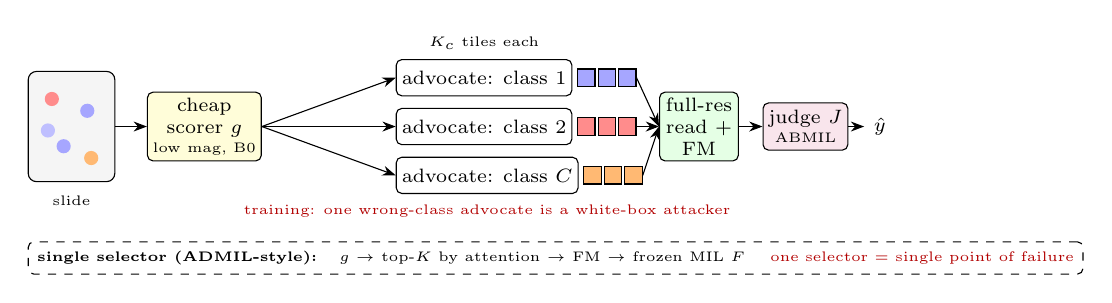
\begin{tikzpicture}[font=\scriptsize, >=Stealth, node distance=2mm,
  box/.style={draw, rounded corners=2pt, align=center, inner sep=2pt, minimum height=6mm},
  tile/.style={draw, minimum size=2.2mm, inner sep=0pt},
  lab/.style={font=\tiny, align=center}]
% slide
\node[draw, rounded corners=3pt, minimum width=11mm, minimum height=14mm, fill=gray!8] (wsi) at (0,0) {};
\foreach \x/\y/\c in {-.25/.35/red!45, .2/.2/blue!35, -.1/-.25/blue!35, .25/-.4/orange!55, -.3/-.05/blue!25}
  \fill[\c] (\x,\y) circle (0.9mm);
\node[lab, below=0.5mm of wsi] {slide};
% cheap scorer
\node[box, fill=yellow!15, right=4mm of wsi] (g) {cheap\\scorer $g$\\[-1pt]{\tiny low mag, B0}};
\draw[->] (wsi) -- (g);
% advocates
\foreach \i/\name/\c/\yy in {1/class 1/blue!35/0.62, 2/class 2/red!45/0, 3/class $C$/orange!55/-0.62} {
  \node[box, minimum width=14mm, minimum height=4.6mm, right=17mm of g.east, anchor=west, yshift=\yy cm] (a\i) {advocate: \name};
  \draw[->] (g.east) -- (a\i.west);
  \foreach \k in {0,1,2} \node[tile, fill=\c, right=0.6mm+\k*2.6mm of a\i.east, anchor=west] (t\i\k) {};
}
\node[lab, above=0mm of a1.north] {$K_c$ tiles each};
\node[font=\tiny, red!70!black] at ($(a3.south)+(0,-0.22)$) {training: one wrong-class advocate is a white-box attacker};
% FM + judge
\node[box, fill=green!10, right=11mm of a2.east, anchor=west, minimum width=10mm] (fm) {full-res\\read +\\FM};
\foreach \i in {1,2,3} \draw[->] (t\i2.east) -- (fm.west);
\node[box, fill=purple!10, right=3mm of fm] (j) {judge $J$\\[-1pt]{\tiny ABMIL}};
\draw[->] (fm) -- (j);
\node[right=2mm of j] (y) {$\hat y$};
\draw[->] (j) -- (y);
% inset: single selector
\node[draw, dashed, rounded corners=2pt, align=left, font=\tiny, anchor=north west] at ($(wsi.south west)+(0,-0.75)$) (inset)
  {\textbf{single selector (ADMIL-style):} \; $g$ $\to$ top-$K$ by attention $\to$ FM $\to$ frozen MIL $F$ \quad {\color{red!70!black}one selector = single point of failure}};
\end{tikzpicture}
}
\caption{\textbf{One advocate per diagnosis.} A cheap scorer reads the slide at low magnification. Each class's advocate presents the $K_c$ tiles that best support its class; only these are read at full resolution and encoded by the foundation model, and the judge compares them. A single selector (dashed box) shows the foundation model one view of the slide.}\label{fig:method}
\end{figure}

%======================================================================
\section{Related work}
\textbf{MIL on foundation-model features.} ABMIL~\cite{ilse2018abmil}, CLAM~\cite{lu2021data}, DSMIL~\cite{li2021dual}, TransMIL~\cite{shao2021transmil} and DTFD-MIL~\cite{zhang2022dtfd} aggregate features of all tiles; with UNI or CONCH features they are the accuracy reference, at full reading and encoding cost.
\textbf{Efficient WSI inference.} ZoomMIL~\cite{thandiackal2022zoommil} learns where to zoom with a differentiable top-$K$, RLogist~\cite{zhao2023rlogist} learns an observation path with reinforcement learning, and ADMIL~\cite{admil2026} and EAGLE~\cite{eagle2026} select a few tiles with a cheap model before running the foundation model. All route the expensive model through one selector; we study its failure mode and when selection pays off.
\textbf{Robustness of MIL.} Adversarial attacks on MIL perturb tile pixels or features~\cite{foote2021now,mil_adv2022}; we instead replace the evidence-selection step, which no pixel-level defence covers.
\textbf{Debate.} Our advocates and judge follow AI-safety debate~\cite{irving2018debate,khan2024debate,kenton2024scalable}, where competing agents present evidence to a weaker judge; here the advocates are cheap and the judge is the expensive model.

%======================================================================
\section{Method}
\textbf{Setting.} A slide is a bag of tiles $\{x_i\}_{i=1}^N$ with label $y\in\{1,\dots,C\}$. Each tile has a cheap view $u_i$ (low magnification, ImageNet EfficientNet-B0) and an expensive view $z_i$ (full resolution, foundation model). A full-slide gated-attention MIL model $F$ on $\{z_i\}$ is the accuracy reference and supervises the cheap scorer.

\textbf{Distilled cheap scorer.} A two-layer MLP $g$ on $u_i$ regresses $F$'s per-tile class logits (standardised) and matches its attention distribution (KL), as in ADMIL~\cite{admil2026}. It is trained on training slides only and never sees the expensive view at test time.

\textbf{Advocates.} Advocate $c$ presents $K_c$ tiles that best support class $c$ under $g$. For subtyping (RCC, NSCLC) these are the top-$K_c$ tiles by margin $g_c(u_i)-\max_{c'\neq c}g_{c'}(u_i)$. For metastasis detection the classes are ordered and advocates follow how each stage presents~\cite{camelyon17}: \emph{negative} shows the least tumour-like tiles; \emph{ITC} the most tumour-like tile and its nearest neighbours; \emph{micro} the most tumour-like tiles within 2\,mm of it; \emph{macro} a farthest-point sample of the top 2\% (CAMELYON16: two advocates, top and bottom tiles). Only the $\sum_c K_c$ presented tiles are read at full resolution and encoded.

\textbf{Judge and adversarial transcripts.} The judge $J$ is a gated-attention MIL model over the presented tiles, each tagged with a one-hot of its advocate. It is warm-started on random tiles, then trained for three rounds on honest transcripts and on transcripts in which the advocate of one wrong class is replaced by a white-box attacker that presents the tiles maximising $J$'s current score for that class.

\textbf{Threat model.} A compromised selector is replaced by a white-box attacker with the same budget that reads every tile with the foundation model (stronger than any cheap selector). For the single selector it presents the $K$ tiles with the highest $F$ score for a wrong class; for ours it replaces one wrong-class advocate (worst case over wrong classes; adaptive and aware of the honest tiles on CAMELYON16).

\textbf{Single-selector baseline.} Our ADMIL-style reimplementation (no code is public) uses the same cheap features and distilled attention head, selects the top-$K$ tiles with $K=\sum_c K_c$, and feeds them to the frozen full-slide model $F$, as in ADMIL.

%======================================================================
\section{Experiments}
\textbf{Data.} \textbf{CAMELYON16}~\cite{c16}: 399 breast lymph-node slides, official split, UNI features (512\,px tiles at 40$\times$, $\sim$12K tiles per slide). \textbf{CAMELYON17}~\cite{camelyon17}: 500 slides from 5 hospitals, 4 node stages (318 negative, 36 ITC, 59 micro, 87 macro), leave-one-hospital-out. \textbf{TCGA-RCC}~\cite{tcga}: 882 primary-tumour diagnostic slides (492 clear cell, 283 papillary, 107 chromophobe). \textbf{TCGA-NSCLC}~\cite{tcga}: 1{,}041 slides (adenocarcinoma vs.\ squamous cell carcinoma). TCGA cohorts use 5-fold patient-level stratified CV. CAMELYON17 and TCGA use CONCH features of 448\,px tiles at 0.5\,\textmu m/px (2.1K--4.5K tiles per slide). The cheap view is EfficientNet-B0 at 112--128\,px from the slide pyramid. $K_c{=}8$ (CAMELYON16) and 4 (others): 16, 16, 12 and 8 encoded tiles per slide.
\textbf{Protocol.} 3 seeds on CAMELYON16, 5 folds $\times$ 3 seeds elsewhere. We report balanced accuracy (BA) and, for the ordinal CAMELYON17 stages, quadratic-weighted $\kappa$.
\textbf{Matched-compute baselines.} \emph{Cheap MIL}: gated ABMIL on B0 features of all tiles (no foundation model). \emph{Random-$K$}: foundation-model ABMIL trained and tested on $K$ random tiles, for $K$ equal to our budget and $4\times$, $16\times$ it. \emph{Escalation}: the least confident 10\% or 20\% of slides are sent to the full-slide model.

\begin{table*}[t]\centering
\caption{\textbf{Clean and compromised-selector results} (mean\pmsd{sd}; 3 runs on CAMELYON16, 15 elsewhere). Attacked: one selector replaced by a white-box attacker. s/slide: measured per-slide wall-clock (A100; Sec.~\ref{sec:cost}).}\label{tab:main}
\setlength{\tabcolsep}{4pt}
\begin{tabular}{@{}lcccccccc@{}}\toprule
 & \multicolumn{2}{c}{CAMELYON16 (BA)} & \multicolumn{2}{c}{CAMELYON17 ($\kappa$)} & \multicolumn{2}{c}{TCGA-RCC (BA)} & \multicolumn{2}{c}{TCGA-NSCLC (BA)}\\\cmidrule(lr){2-3}\cmidrule(lr){4-5}\cmidrule(lr){6-7}\cmidrule(l){8-9}
method & clean & attacked & clean & attacked & clean & attacked & clean & attacked\\\midrule
full-slide MIL (all tiles) & .969\pmsd{.008} & -- & .890\pmsd{.054} & -- & .933\pmsd{.016} & -- & .923\pmsd{.019} & -- \\
single selector (ADMIL-style) & .943\pmsd{.014} & .315\pmsd{.059} & .873\pmsd{.089} & $-$.241\pmsd{.237} & .907\pmsd{.036} & .022\pmsd{.014} & .909\pmsd{.017} & .003\pmsd{.004}\\
\textbf{advocates (ours)} & .942\pmsd{.010} & \textbf{.931}\pmsd{.013} & .823\pmsd{.105} & \textbf{.715}\pmsd{.152} & .920\pmsd{.028} & \textbf{.866}\pmsd{.029} & .874\pmsd{.019} & \textbf{.841}\pmsd{.015}\\\midrule
encoded tiles / slide & \multicolumn{2}{c}{16 of $\sim$12K} & \multicolumn{2}{c}{16 of 2.1K} & \multicolumn{2}{c}{12 of 4.5K} & \multicolumn{2}{c}{8 of 4.0K}\\
s/slide: full $\to$ selective & \multicolumn{2}{c}{33.3 $\to$ 5.5 (6.1$\times$)} & \multicolumn{2}{c}{24.4 $\to$ 6.7 (3.6$\times$)} & \multicolumn{2}{c}{32.4 $\to$ 7.9 (4.1$\times$)} & \multicolumn{2}{c}{26.3 $\to$ 6.6 (4.0$\times$)}\\\bottomrule
\end{tabular}\end{table*}

\begin{figure}[t]\centering
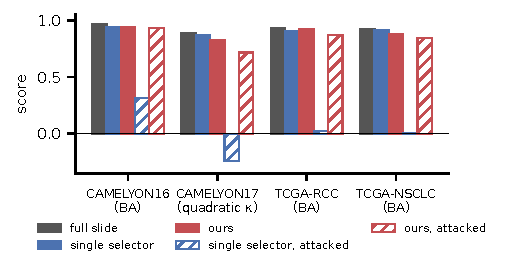
\includegraphics[width=\columnwidth]{figs/fig_robust.pdf}
\caption{\textbf{A single selector is a single point of failure.} Clean (solid) and compromised-selector (hatched) scores. The single-selector pipeline falls to or below chance on every dataset; advocates lose 1--11 points.}\label{fig:robust}
\end{figure}

\subsection{A single selector is a single point of failure}
On clean slides the single selector is a strong baseline: within 1.4--2.6 points of full-slide MIL while encoding 0.2--0.8\% of tiles (Table~\ref{tab:main}). When it is compromised it falls to .315 BA on CAMELYON16, $-$.241 $\kappa$ on CAMELYON17, .022 BA on RCC and .003 BA on NSCLC, i.e.\ it is steered to the attacker's class on almost every slide, in every fold and seed. Under the same attack advocates keep .931, .715, .866 and .841 and are ahead of the single selector in every run (3/3 on CAMELYON16, 15/15 on each other dataset; paired slide-level bootstrap $p<.001$ on all four; Fig.~\ref{fig:robust}). Robustness does not come from redundancy alone: showing the \emph{frozen} full-slide model the single selector's tiles together with an adaptive attacker's tiles (no adversarial judge training) gives .878 BA on CAMELYON16 (ours .931).

On clean slides advocates match the single selector on CAMELYON16 (.942 vs.\ .943), are level on RCC (.920 vs.\ .907, $p=.09$) and significantly behind on CAMELYON17 ($-$5.0\,$\kappa$ points) and NSCLC ($-$3.5 points; both $p<.001$). The next section shows that on the two TCGA tasks neither selector is the right tool.

\begin{figure*}[t]\centering
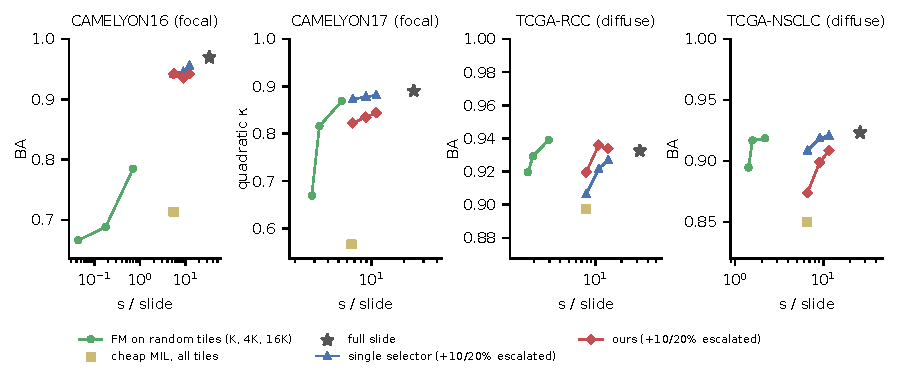
\includegraphics[width=\textwidth]{figs/fig_frontier.pdf}
\caption{\textbf{When does cheap selection matter?} Score vs.\ measured per-slide wall-clock (log scale). Green: foundation model on $K$, $4K$, $16K$ random tiles (trained on random tiles). Lines for the selectors go from selective inference to escalating the least confident 10\% and 20\% of slides to the full-slide model. On focal metastasis tasks (left) random tiles fail and selection is required; on diffuse subtyping tasks (right) a few random tiles match every selector at a quarter of the cost. CAMELYON16 tiling time was not measured, so its random-tile cost is a lower bound.}\label{fig:frontier}
\end{figure*}

\subsection{When does cheap selection matter?}\label{sec:frontier}
Fig.~\ref{fig:frontier} places every method on the accuracy--cost plane.

\textbf{Focal disease needs selection.} A lymph-node metastasis can occupy a fraction of a percent of the slide. With our budget, random tiles reach .666 BA on CAMELYON16 and .669 $\kappa$ on CAMELYON17, and even 16$\times$ the budget (256 tiles) reaches only .785 and .869. A cheap MIL model on all tiles is worse still (.713, .567): low-magnification features alone cannot stage a node. Both selectors are 25--28 points above random tiles at equal budget, so on these tasks the efficient pipeline depends entirely on its selector---exactly where a single point of failure is most costly.

\textbf{Diffuse disease does not.} RCC and NSCLC subtype is visible almost everywhere in the tumour. Twelve random CONCH tiles reach .920 BA on RCC (= ours, $>$ the single selector) and 8 reach .895 on NSCLC; 192 and 32 random tiles reach .939 and .917, matching full-slide MIL. Random sampling needs no cheap pass over the slide, so it costs 1.4--2.9\,s per slide, about a quarter of either selector. On these tasks we recommend random sampling, which also has no selector to compromise.

\textbf{Escalation.} Sending the least confident 10\% of slides to the full model costs $\sim$2--3\,s per slide on average. It closes most of the gap for the single selector (CAMELYON16 .946, CAMELYON17 .878) and for ours on RCC (.936, error-detection AUROC .90), but our confidence is a weaker error signal on CAMELYON17 (.835).

\subsection{Cost}\label{sec:cost}
We time each stage during feature extraction on an A100 (mean over every third slide). Full-slide inference = tissue tiling + full-resolution read of all tiles + foundation model: 24--33\,s per slide, of which reading is 19--26\,s and the foundation model 2.4--10.8\,s. Selective inference = tiling + low-magnification read (2.6--4.7\,s) + B0 (1.2--1.5\,s) + reading and encoding the presented tiles ($<$0.3\,s): 5.5--7.9\,s, a 3.6--6.1$\times$ speed-up. Advocates and the single selector have identical cost at equal $K$. The low-magnification read is now the bottleneck, so storing a low-resolution copy of each slide would cut cost further.

\subsection{Ablations and negative results}
\begin{table}[t]\centering
\caption{\textbf{Ablations} (clean / attacked). No flags: judge without presenter identity. Tiles$\to F$: advocate tiles fed to the frozen full-slide model.}\label{tab:abl}
\setlength{\tabcolsep}{2.5pt}
\begin{tabular}{@{}lcccc@{}}\toprule
 & C16 BA & C17 $\kappa$ & RCC BA & NSCLC BA\\\midrule
ours & .942/.931 & .823/.715 & .920/.866 & .874/.841\\
\ \ no flags & .937/.923 & .826/.719 & .925/.867 & .875/.838\\
\ \ tiles$\to F$ & -- & -- & .911/-- & .868/--\\
single sel. & .943/.315 & .873/$-$.241 & .907/.022 & .909/.003\\\bottomrule
\end{tabular}\end{table}
\textbf{Presenter identity is not needed} (Table~\ref{tab:abl}): a judge without advocate flags, trained the same way, is as accurate and as robust; the gains come from per-class selection plus adversarial judge training. \textbf{Per-class selection alone is not enough}: advocate tiles fed to the frozen full-slide model are no better than the single selector on clean slides (.911 RCC, .868 NSCLC). \textbf{Natural stain shift does not break the single selector}: a random HED perturbation~\cite{tellez2019stain} of the cheap view of CAMELYON17 test slides costs both methods $\le$3 points (single selector .892$\to$.874, ours .815$\to$.790, seed 0). The failure we study is a wrong or compromised selector, not routine staining variation.

\textbf{Limitation: isolated tumour cells.} Every low-magnification method misses the smallest metastases on CAMELYON17: ITC recall is .03 for both selectors (full-slide MIL .30) and micrometastasis recall .25 (ours) and .36 (single selector) vs.\ .64. The clean $\kappa$ gap to full-slide MIL comes from these stages; finding them needs a higher-resolution cheap view or escalation.

%======================================================================
\section{Discussion and conclusion}
Efficient WSI pipelines that route the foundation model through one cheap selector are accurate when the selector is right and fail completely when it is not. Giving each candidate diagnosis its own advocate and training the judge against one adversarial advocate keeps the cost of selective inference and removes that failure mode on all four datasets. Matched-compute baselines show where this matters: focal tasks such as lymph-node metastasis depend entirely on the selector, while diffuse subtyping tasks are better served by random sampling. \textbf{Limitations.} Advocates do not improve clean accuracy over the single selector and trail it on CAMELYON17 and NSCLC; our single selector is a reimplementation; the threat model is a worst-case white-box replacement rather than an observed real-world failure; and no cheap method finds isolated tumour cells. \textbf{Future work.} Cervical cytology screening, where a few abnormal cells among $\sim$10$^5$ decide the diagnosis, is a natural focal task; \todo{Dr.\ Zhou cohort, if available}.

{\small
\bibliographystyle{unsrt}
\bibliography{refs}}
\end{document}
